\documentclass[12pt,a4paper]{report}

\usepackage[italian]{babel}
\usepackage{newlfont}
\usepackage[latin1]{inputenc}
\usepackage{csquotes}
\usepackage{fancyhdr}
\usepackage{indentfirst}
\usepackage{graphicx} %%%%libreria per utilizzare i grafici
\usepackage{newlfont} %libreria per utilizzare font particolari
%librerie matematiche
\usepackage{amssymb}
\usepackage{amsmath}
\usepackage{latexsym}
\usepackage{amsthm}
\usepackage{hyperref}   %%TODO: posso metterla?
%%BIBLIOGRAPHY  
\usepackage{biblatex}

%fancyhdr
\usepackage{fancyhdr}
\pagestyle{fancy}
\chead{}
\rhead{\thepage}
\renewcommand{\headrulewidth}{0.4pt}
\renewcommand{\footrulewidth}{0.4pt}
\setlength{\headheight}{27.1pt}

%lstset
\usepackage{listings}
\lstset{
    basicstyle=\footnotesize\ttfamily,
    % specifies that lines shouldn't overrun the margin
    breaklines=true
    % specified that, if possible, lines should be broken at whitespace
    breakatwhitespace=true 
}

%images
\usepackage{float}

\hypersetup{
pdftitle={Metodologie di attacco ai Large Language Models},
pdfauthor={Enrico Ferraiolo}
}

\addbibresource{bib.bib}

%\textwidth=450pt\oddsidemargin=0pt

\begin{document}

%frontespizio
\begin{titlepage}
\begin{center}
{{\Large{\textsc{Alma Mater Studiorum $\cdot$ Universit\`a di
Bologna}}}} \rule[0.1cm]{15.8cm}{0.1mm}
\rule[0.5cm]{15.8cm}{0.6mm}
{\small{\bf SCUOLA DI SCIENZE\\
Corso di Laurea in Informatica }}
\end{center}
\vspace{15mm}
\begin{center}
{\LARGE{\bf Metodologie di attacco ai}}\\
%\vspace{3mm}
%{\LARGE{\bf ai}}\\
\vspace{3mm}
{\LARGE{\bf Large Language Models}}\\
\end{center}
\vspace{40mm}
\par
\noindent
\begin{minipage}[t]{0.47\textwidth}
{\large{\bf Relatore:\\
Chiar.mo Prof.\\
ANDREA ASPERTI}}
\end{minipage}
\hfill
\begin{minipage}[t]{0.47\textwidth}\raggedleft
{\large{\bf Presentata da:\\
ENRICO FERRAIOLO}}
\end{minipage}
\vspace{20mm}
\begin{center}
{\large{\bf II Sessione\\%inserire il numero della sessione in cui ci si laurea
Anno Accademico 2023-2024}}%inserire l'anno accademico a cui si è iscritti
\end{center}
\end{titlepage}

%dedica
\begin{titlepage}                       %crea un ambiente libero da vincoli
                                        %   di margini e grandezza caratteri:
                                        %   si pu\`o modificare quello che si
                                        %   vuole, tanto fuori da questo
                                        %   ambiente tutto viene ristabilito
%
\thispagestyle{empty}                   %elimina il numero della pagina
\topmargin=6.5cm                        %imposta il margina superiore a 6.5cm
\raggedleft                             %incolonna la scrittura a destra
\large                                  %aumenta la grandezza del carattere
                                        %   a 14pt
\em                                     %emfatizza (corsivo) il carattere
A mio fratello\\Francesco                %\ldots lascia tre puntini
\newpage                                %va in una pagina nuova
%
%%%%%%%%%%%%%%%%%%%%%%%%%%%%%%%%%%%%%%%%
\clearpage{\pagestyle{empty}\cleardoublepage}%non numera l'ultima pagina sinistra
\end{titlepage}


\pagenumbering{roman}                   %serve per mettere i numeri romani

%% ABSTRACT
\clearpage
\thispagestyle{empty}
\hfill
\clearpage
\section*{Abstract}
Negli ultimi anni, i \emph{Large Language Model} (LLM) hanno rappresentato una rivoluzione nell'elaborazione del linguaggio naturale grazie alle loro capacit\`a generative e alla comprensione del contesto. Tuttavia questi modelli sono vulnerabili a diversi tipi di attacchi che possono comprometterne la sicurezza e l'affidabilit\`a.\\
Questo studio vuole formalizzare il concetto degli attacchi ai \emph{Large Language Model} dando una caratterizzazione matematica al problema.\\
Gli esperimenti condotti dimostrano la facilit\`a con cui tali attacchi possono manipolare il comportamento del modello, evidenziando rischi per l'integrit\`a e la sicurezza per i proprietari e gli utilizzatori.\\
Questa tesi, inoltre, affronta ed esplora le principali metodologie di attacco ai LLM sperimentando approfonditamente le tecniche di \emph{Prompt Injection} e \emph{Data Poisoning}.
\clearpage
\thispagestyle{empty}
\hfill
\clearpage

\clearpage{\pagestyle{empty}\cleardoublepage}

\tableofcontents                        %crea l'indice
\listoffigures  

\pagenumbering{arabic}                  %mette i numeri arabi

%introduzione
\chapter{Introduzione}
Negli ultimi anni i \emph{Large Language Model} (LLM) sono stati una delle pi\`u grandi innovazioni nel campo del \emph{Natural Language Processing} (NLP). Questi modelli linguistici sono basati su architetture come i \emph{Transformer}. Sono in grado di elaborare e generare testo in linguaggio naturale simulando un dialogo umano. Grazie alle loro forti capacit\`a di analisi di contesti complessi e di risposta coerente alla conversazione i LLM sono stati adottati in numerosi settori e campi, ci\`o per\`o implica anche una maggiore preoccupazione in ambito di sicurezza poich\`e aumenta il rischio di \emph{fooling}.\\

Il concetto di \emph{fooling} fa riferimento alla capacit\`a di indurre un modello a comportarsi in modo inatteso producendo output errati, incoerenti o addirittura pericolosi. Non \`e banale la differenza tra \emph{fooling} sulle \emph{Deep Neural Network} (DNN) e \emph{fooling} sui LLM, infatti il primo si basa principalmente sulla manipolazione  dell'input del modello di classificazione per ottenere una risposta erroneamente classificata, sfruttando le vulnerabilit\`a legate alla rappresentazione delle \emph{feature}. Fare \emph{fooling} su \emph{Large Language Model}, invece, il problema \`e decisamente pi\`u complicato e questo tema verr\`a approfondito nel corso della tesi.\\
La natura del problema appena descritto lascia la strada aperta a numerose forme diverse di attacco, a seconda degli obiettivi e delle modalit\`a di accesso al modello. Questo lavoro tenta di dare una formalizzazione al problema cercando di generalizzare un attacco a un modello linguistico.\\

Per comprendere a pieno l'impatto che hanno sulla realt\`a gli attacchi si \`e rivelato molto utile condurre esperimenti pratici. Questi sono stati progetti e realizzati per verificare le tecniche di \emph{fooling} descritte in questo lavoro.\\

\`E quindi chiaro che questa tesi non cerca solo di analizzare la teoria alla base degli attacchi e darne formalizzazione matematica, ma anche di tradurre tali concetti in esperimenti pratici cercando di esplorare le implicazioni di sicurezza per i \emph{Large Language Model}.

%llm
\chapter{Large Language Model}
\section{Introduzione ai LLM}
I \emph{Language Model} (LM) sono modelli linguistici, basati sul \emph{machine learning}, che vengono addestrati su quantit\`a enormi di dati e per questo vengono chiamati \emph{Large Languge Model}, essi generano ed elaborano testo in linguaggio naturale. \\
Negli ultimi tempi il campo del \emph{Natural Language Processing} (NLP) si \`e evoluto con una rapidit\`a molto elevata, questo grazie a tutte le ricerche fatte e i progressi ottenuti in ambito scientifico e tecnologico. 
Il NLP \`e un'area di studio che fa convergere informatica, intelligenza artificiale e linguistica, l'obiettivo \`e quello di far elaborare a una macchina del testo in linguaggio naturale, "capirne" il significato e coglierne le sfumature emotive \cite{blaise2022llmunderstandus}.\\
In passato i LLM erano costruiti attraverso le \emph{Recurrent Neural Network}, (RNN) pi\`u precisamente mediante un'architettura nota come \emph{Long short-term memory} (LSTM) il cui obiettivo \`e quello di ridurre il problema della scomparsa del gradiente presente nelle RNN.
Al giorno d'oggi lo stato dell'arte \`e diverso, infatti troviamo che i modelli pi\`u performanti sono quelli basati sui \emph{Transformer} \cite{vaswani2023attentionneed}.

\section{Transformer}
Un \emph{Transformer}, di norma, \`e composto da un \emph{encoder} e un \emph{decoder}, figura \ref{fig:architetturaTransformer}, entrambe le parti sono composte da \emph{layer} fortemente connessi.
Esso prende in input del testo in linguaggio naturale e lo rielabora trasformandolo in una rappresentazione numerica composta da sequenze di token.
\begin{figure}[H]
    \centering
    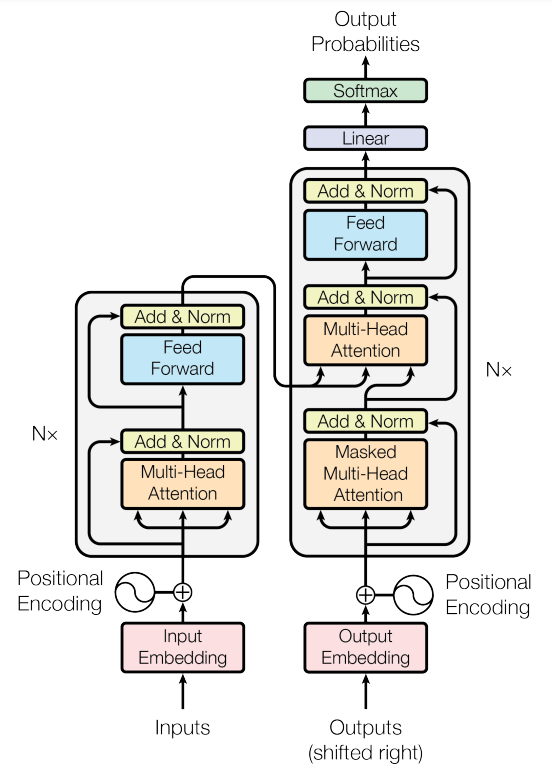
\includegraphics[width=0.4\textwidth]{media/1-introduzioneLLM/thetransformerarchitecture.png}
    \caption{L'architettura di un \emph{Transformer}. Immagine presa da \cite{vaswani2023attentionneed}.}
    \label{fig:architetturaTransformer}
\end{figure}

I \emph{Transformer} basano la loro forza sulla \emph{Self-Attention}, questo \`e un meccanismo che permette di creare collegamenti globali tra l'input e l'output, ci\`o ha permesso di liberarsi dall'uso delle \emph{recurrent unit} presenti nelle RNN. Queste unit\`a fungevano da memoria il quale valore riceveva un aggiornamento per ogni passo eseguito durante l'apprendimento della rete, questa modalit\`a di aggiornamento dei valori \`e fortemente inefficiente rispetto alla tecnica della \emph{Self-Attention}.

\subsection{Funzionamento e Self-Attention}
La \emph{Self-Attention} \`e il meccanismo chiave per il funzionamento dell'architettura \emph{Transformer}. Questa tecnologia consente al modello di considerare ed esaminare contemporaneamente l'intera sequenza di token ricevuta in input, contrariamente a quanto fanno le RNN, che elaborano i dati sequenzialmente.
Inoltre \emph{Self-Attention} riesce ad attribuire a ogni token un valore che rappresenta la rilevanza di questo all'interno dell'input.\\
Quando viene dato al \emph{Transformer} un input, come ad esempio una frase in linguaggio naturale, questo lo prende e lo rappresenta come una sequenza di numeri. Quest'operazione si chiama \emph{embedding}, ed \`e la pratica di associare ad ogni token un numero e creare un vettore di numeri, cosicch\'e il modello riesca a lavorare effettivamente su dei numeri, interpretabili correttamente dalla rete, e non su del testo.\\
A questo punto possiamo calcolare l'\emph{attention} attraverso un prodotto scalare come nella figura \ref{fig:scaledDotProductAttention}:
\begin{figure}[H]
    \centering
    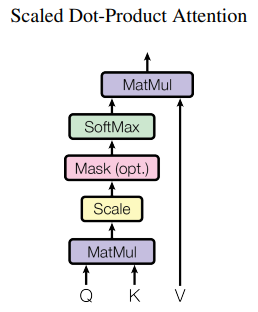
\includegraphics[width=0.4\textwidth]{media/1-introduzioneLLM/scaledDotProductAttention.png}
    \caption{Calcolo dell'\emph{attention} attraverso il prodotto scalare. Immagine presa da \cite{vaswani2023attentionneed}.}
    \label{fig:scaledDotProductAttention}
\end{figure}

\[\text{Attention}(Q,K,V)=\text{softmax}(\frac{QK^T}{\sqrt{d_k}})V\]
dove \(Q\) \`e la matrice delle query da elaborare,
\(K\) \`e la matrice delle chiavi e \(V\) e la matrice dei valori.\\
Un grande vantaggio che implementano i \emph{Transformer} \`e quello della parallelizzazione del calcolo dell'\emph{attention}, infatti attraverso la \emph{Multi-Head Attention} \`e possibile eseguire in parallelo pi\`u istanze della funzione \textsc{Attention} e concatenarne i risultati, come nella figura \ref{fig:multiHeadAttention}. Ci\`o rende i \emph{Transformer} incredibilmente pi\`u efficienti rispetto alle RNN.
\begin{figure}[H]
    \centering
    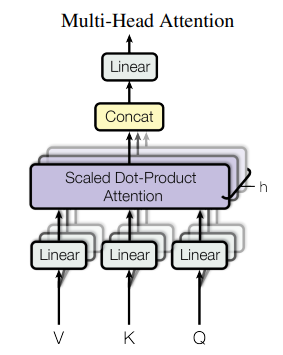
\includegraphics[width=0.4\textwidth]{media/1-introduzioneLLM/multiHeadAttention.png}
    \caption{\emph{Multi-Head Attention}. Immagine presa da \cite{vaswani2023attentionneed}.}
    \label{fig:multiHeadAttention}
\end{figure}

\section{A Che Cosa Servono i LLM}
Lo stato dell'arte dei LLM include diversi modelli, alcuni sono \emph{open source} altri invece no.
Tra i modelli pi\`u popolari e performanti troviamo:
\begin{itemize}
    \item ChatGPT 4o \cite{openaihellogpt4o}
    \item LLaMa 3 \cite{dubey2024llama3herdmodels}
    \item Mistral Large 2 \cite{mistralaimistrallarge2}
    \item Claude 3.5 Sonnet \cite{anthropicclaude35sonnet}
\end{itemize}
Questi modelli sono altamente potenti e in grado di elaborare e generare testo in linguaggio naturale, molti sono anche multi-modali: ovvero riescono a ricevere degli input diversi dal semplice linguaggio naturale, come ad esempio immagini, video oppure altri tipi di documenti.
Il grande punto di forza dei \emph{Large Language Model} risiede nel cogliere le varie sfaccettature che rendono unico ogni tipo di input, capirne il contesto ed elaborare una risposta coerente con le richieste.
Tutto ci\`o rende fortemente utili i LLM, infatti nell'ultimo periodo hanno raggiunto lo status di assistenti virtuali i quali riescono a completare con successo quasi tutte le richieste di un utente medio che si interfaccia a essi. Esistono per\`o delle tecniche di \emph{fooling} che permettono di compromettere l'affidabilit\`a e la sicurezza di questi modelli, anche dei pi\`u avanzati. Bisogna perci\`o sapere come usarli e i proprietari di questi modelli devono essere in grado di difendersi dai pericoli che ne derivano per loro e per i loro clienti.


%fooling
\chapter{Fooling di LLM}
\section{Cosa Vuole Dire Fare Fooling}
Fare \emph{fooling} di un LLM significa indurre il modello a produrre errori generando output non accurati, offensivi o pericolosi attraverso degli input architettati ad hoc per far cadere in inganno il modello linguistico. Tali attacchi sono possibili poich\`e si vanno ad attaccare le vulnerabilit\`a del modello e la sua architettura. L'addestramento dei LLM avviene su enormi quantit\`a di dati e questo comporta l'esposizione del modello in questione a informazioni particolarmente sensibili, contenuti offensivi e notizie false.
Il modello quindi, nonostante sia stato addestrato su una notevole mole di dati utili, ha comunque imparato dei concetti che non dovrebbero essere esposti all'utente finale, \`e quindi chiaro il pericolo che ne concerne e che bisogna attivare delle tecniche di difesa da utenti malintenzionati e/o possibili fughe di dati dal modello mentre sta elaborando una risposta.\\
Ne consegue quindi che fare \emph{fooling} non \`e solamente l'atto di sfruttare una debolezza del modello per il proprio interesse, ma anzi pu\`o voler stare a significare semplicemente portare il \emph{Language Model} a non comportarsi nella modalit\`a attesa.\\
Nel prossimo capitolo vediamo alcune tipologie di attacchi che si possono eseguire sui LLM.





\section{Fooling}
\`E fondamentale sottolineare che il \emph{fooling} nei modelli generativi, e in particolar modo nei LLM, presenta sfide pi\`u complicate rispetto agli attacchi a delle reti di classificazione. In queste ultime la sfida del \emph{fooling} \`e evidente poich\'e, spesso, l'obiettivo \`e quello di fare categorizzare in modo sbagliato, possibilmente con alta fiducia, a un modello un certo input.\\
Nel contesto dei \emph{Large Language Model} , invece, il \emph{fooling} \`e ancora pi\`u complesso. I modelli linguistici, infatti, non devono semplicemente classificare l'input, ma bens\`i devono generare testo in un dominio enorme. \`E quindi chiaro che il \emph{fooling} di un LLM non si limita solamente alla produzione di output errati, ma si espande anche al far generare testo al modello che risulta pericoloso oppure incoerente rispetto al contesto in questione. L'attacco dovr\`a anche tenere quindi conto della comprensione semantica e pragmatica che il modello ha appresso.\\
Nonostante la loro natura generativa, il \emph{fooling} di LLM risulta pi\`u complicato rispetto a quello dei modelli di classificazione tradizionali, questo perch\'e gli ultimi si limitano a produrre output senza tener conto delle difficolt\`a linguistiche a cui si affacciano i LLM, essi infatti si trovano a dover affrontare sfide come ambiguit\`a, contesto e coerenza narrativa durante il discorso.

%attacco
\chapter{Attacco}
% TODO: da mettere
% \section{Motivazioni attacco}
% magari questo lo posso mettere nelle conclusioni? o va bene qui?

Prima di approfondire il significato di attacco a un \emph{Large Language Model} vediamo come si possono attaccare i modelli di \emph{machine learning}, in particolare poniamo la nostra attenzione sulle \emph{Deep Neural Network}.

\section{Attaccare le Deep Neural Network}
%%%%%%%%%%%%%%%
\subsection{Propriet\`a Contro-intuitive delle DNN}
Szegedy et al. \cite{intriguing13} hanno trovato delle propriet\`a contro-intuitive nelle \emph{Deep Neural Network} che risultano particolarmente interessanti per quanto concerne il tema del \emph{fooling} delle reti di \emph{deep learning}, compresi i LLM.

\subsubsection{Rilevazione delle Informazioni Semanticamente Significative}
% La prima propriet\`a individuata riguarda il significato semantico delle unit\`a individuali: \`e infatti stato notato che, contrariamente a quanto si pu\`o immaginare, non \`e il singolo neurone nell'ultimo strato a contenere informazioni semantiche significative rispetto all'input, ma bens\`i, a contenerle, \`e lo spazio d'attivazione nella sua interezza.\\
% \`E stato provato tramite un esperimento che proiezioni casuali delle attivazioni \(\phi(x)\), dove \(\phi(x)\) \`e la funzione di attivazione delle \emph{feature} estratte dal modello per un input \(x\), sono semanticamente indistinguibili dalle coordinate di \(\phi(x)\). Ci\`o mette in discussione l'idea che le reti neurali separino le caratteristiche nei singoli neuroni.
La prima propriet\`a scoperta riguarda il significato semantico delle unit\`a individuali: non \`e il singolo neurone nell'ultimo strato a contenere informazioni semantiche significative, ma bens\`i l'intero spazio di attivazione.\\
\`E stato provato tramite un esperimento che proiezioni casuali delle attivazioni \(\phi(x)\), dove \(\phi(x)\) \`e la funzione di attivazione delle \emph{feature} estratte dal modello per un input \(x\), sono semanticamente indistinguibili dalle coordinate di \(\phi(x)\). Questo mette in discussione l'idea che le reti neurali separino le caratteristiche nei singoli neuroni.

\subsubsection{Perturbazione dell'Input}
% La seconda propriet\`a rilevata riguarda la stabilit\`a delle DNN in risposta a minime perturbazioni sugli input. \`E infatti stato notato che impercettibili (ad occhio nudo) e non casuali cambiamenti su un'immagine di input modificano arbitrariamente la classificazione di questa da parte del modello, inducendolo a sbagliare. Queste perturbazioni sono trovate ottimizzando l'input e massimizzando l'errore predetto, tali input perturbati vengono chiamati \emph{adversarial example}.\\
% Ci\`o che \`e stato appena descritto \`e un metodo di attraversare il \emph{manifold} in modo efficiente (tramite l'ottimizzazione) e trovare degli \emph{adversarial example} nello spazio degli input. Inoltre viene anche mostrato che tali \emph{adversarial example} sono comuni ad altre reti, infatti una perturbazione progettata per una rete potrebbe ingannare anche altri modelli, addestrati con configurazioni diverse o addirittura dataset differenti, sullo stesso input.
Un'altra propriet\`a riguarda la vulnerabilit\`a a minime perturbazioni dell'input: cambiamenti impercettibili su un'immagine di input possono indurre il modello a classificazioni completamente errate. Tali perturbazioni, ottimizzate per massimizzare l'errore predetto, vengono chiamate \emph{adversarial example}.\\
Viene anche mostrato che tali \emph{adversarial example} sono comuni ad altre reti, infatti una perturbazione progettata per una rete potrebbe ingannare anche altri modelli, addestrati con configurazioni diverse o addirittura su dataset differenti, sullo stesso input.\\
Un esempio pratico di questa propriet\`a lo possiamo notare nella figura \ref{fig:intriguing_adv_example} dove troviamo degli \emph{adversarial examples} progettati per una \emph{AlexNet}: sulla sinistra ci sono gli input originali, al centro la differenza tra l'immagine corretta e quella ostile mentre sulla colonna di destra c'\`e l'\emph{adversarial example}. Tutte le immagini sulla destra sono classificate come "struzzo".

\begin{figure}[H]
    \centering
    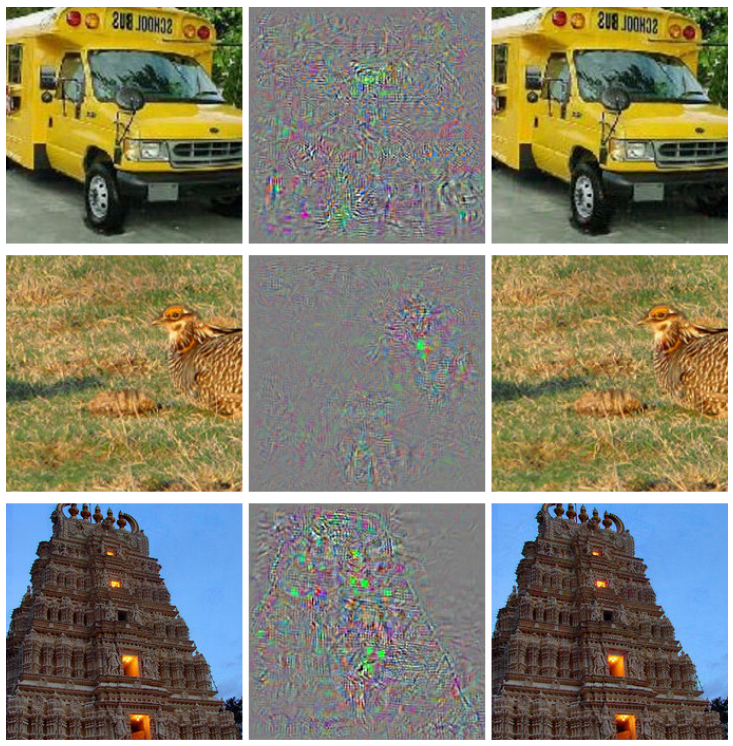
\includegraphics[width=0.4\textwidth]{media/2-fooling/adversarial_examples_intruguing13.png}
    \caption{\emph{Adversarial examples}. Immagine presa da \cite{intriguing13}.}
    \label{fig:intriguing_adv_example}
\end{figure}
%%%%%%%%%%%%%%%
%%%%%%%%%%%%%%%
\subsection{Alta Confidenza nella Classificazione di Immagini Irriconoscibili}
Nguyen et al. \cite{blackbox_fool15} presentano un articolo dove discutono del fatto che le DNN sono vulnerabili ad attacchi che portano a classificazioni errate e con alta fiducia per input completamente estranei e non riconoscibili da un occhio umano.

\subsubsection{Creazione delle Fooling Image}
% Le \emph{fooling image} sono immagini generate appositamente per portare la rete a classificare in modo errato come oggetti specifici.\\
% Per la creazioni di queste immagini gli autori dell'articolo hanno utilizzato algoritmi evolutivi o tramite la tecnica dell'ascesa del gradiente. L'obiettivo era quello di manipolare i pixel dell'immagine in modo tale da massimizzare la risposta della rete per una determinata classe. Vengono inoltre utilizzati due tipi di codifica per la generazione degli input ostili: 
% \begin{itemize}
%     \item Codifica diretta
%     \item Codifica indiretta
% \end{itemize}
% Nella codifica diretta ogni pixel \`e rappresentato da un valore e l'evoluzione avviene mutando tali valori pixel per pixel, producendo immagini irregolari.\\
% Nella codifica indiretta, invece, viene usata una rete CPPN (\emph{Compositional Pattern-Producing Network}) che genera l'intera l'immagine. In questo approccio ogni genoma influenza parti diverse dell'immagine, producendo risultati con una maggiore regolari\`a e coerenza visiva.\\
% Per esempio nella figura \ref{fig:direct_encoding_example} viene usata la codifica diretta. Il modello classifica tali immagini con una confidenza del 99,99\% come cifre da 0 a 9. Nella figura \ref{fig:indirect_encoding_example} invece possiamo trovare un esempio per la codifica indiretta, possiamo subito notare che le immagini sono molto pi\`u regolari rispetto alle precedenti e la rete classifica con una confidenza del 99,99\% le immagini come cifre da 0 a 9.

Le \emph{fooling image} sono immagini generate appositamente per portare la rete a classificare in modo errato l'input come un oggetto specifico.\\
Per la creazioni di queste immagini gli autori dell'articolo hanno utilizzato algoritmi evolutivi e tecniche come l'ascesa del gradiente. L'obiettivo era quello di manipolare i pixel dell'immagine in modo tale da massimizzare la risposta della rete per una determinata classe. Vengono inoltre utilizzati due tipi di codifica per la generazione degli input ostili: 
\begin{itemize}
    \item \textbf{Codifica diretta}: ogni pixel \`e rappresentato da un valore e l'evoluzione avviene mutando tali valori pixel per pixel, producendo immagini irregolari.
    \item \textbf{Codifica indiretta}: viene usata una rete CPPN (\emph{Compositional Pattern-Producing Network}). Ogni genoma influenza parti diverse dell'immagine, producendo risultati con una maggiore regolari\`a e coerenza visiva.
\end{itemize}
Per esempio, per la creazione delle \emph{fooling image}, nella figura \ref{fig:direct_encoding_example} viene usata la codifica diretta e nella figura \ref{fig:indirect_encoding_example} viene usata la codifica indiretta. La rete, in entrambi i casi, classifica le immagini come cifre da 0 a 9.

\begin{figure}[H]
    \centering
    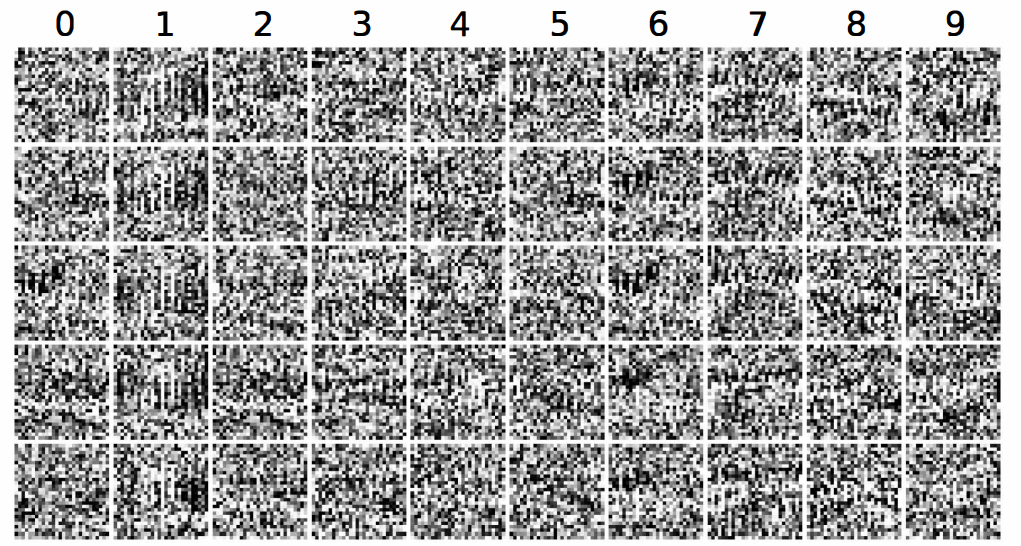
\includegraphics[width=0.4\textwidth]{media/2-fooling/deep_neural_networks_are_easily_fooled_direct_encoding_example.png}
    \caption{Codifica diretta. Immagine presa da \cite{blackbox_fool15}.}
    \label{fig:direct_encoding_example}
\end{figure}
\begin{figure}[H]
    \centering
    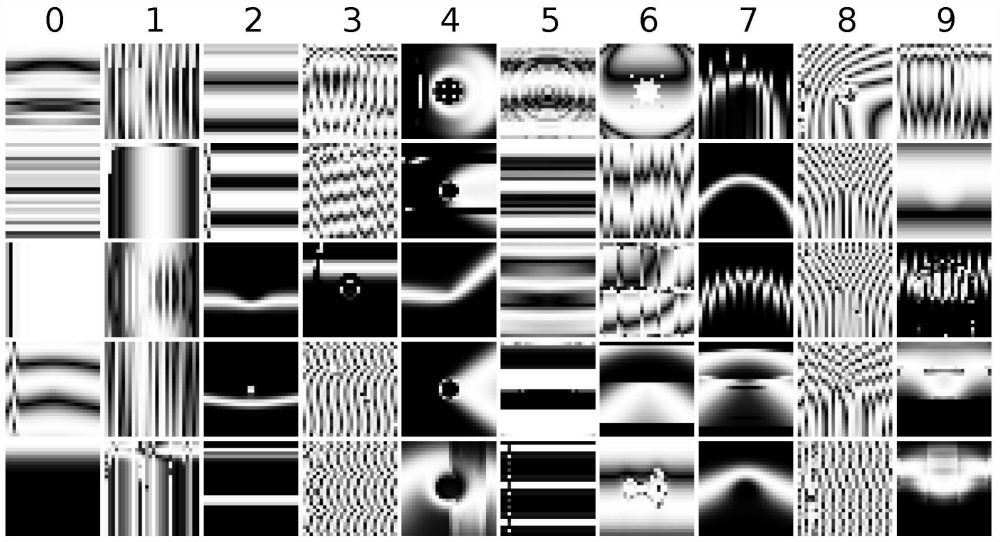
\includegraphics[width=0.4\textwidth]{media/2-fooling/deep_neural_networks_are_easily_fooled_indirect_encoding_example.png}
    \caption{Codifica indiretta. Immagine presa da \cite{blackbox_fool15}.}
    \label{fig:indirect_encoding_example}
\end{figure}
%%%%%%%%%%%%%%%%%%%%%%%%%%%%%%%%

\section{Cosa Vuole Dire Attaccare un LLM}
Un attacco a un \emph{Large Language Model} \`e un tentativo intenzionale di manipolare l'output generato dal modello, attraverso lo sfruttamento di vulnerabilit\`a e debolezze al fine di ottenere risposte che soddisfino gli obiettivi malevoli oppure indesiderati voluti da un utente minaccioso.\\
Questi attacchi spaziano dall'elusione dei filtri di sicurezza della rete fino all'induzione di risposte che non sono coerenti con quelle aspettate.\\
Nei modelli di classificazione gli attacchi si concentrano tipicamente sull'induzione di errori nella classificazione della classe attraverso minime perturbazioni sull'input, affinch\'e il modello associ erroneamente un input malevolo come appartenente a una classe benigna (ad esempio facendo associare un immagine di un veicolo come un animale). La classificazione di tale attacco \`e abbastanza semplice, infatti un attacco ha successo se l'output del classificatore risulta errato rispetto alla \emph{ground truth}.\\
Nei modelli generativi, invece, la natura dell'output \`e per l'appunto di tipo generativa e questo rende notevolmente pi\`u complessa la misurazione del successo di un attacco. In questi modelli l'attaccante non si limita a forzare la classificazione erronea di una classe, ma invece cerca di influenzare l'output generato in modo tale che questo contenga informazioni che violino i criteri di sicurezza della rete oppure che non sarebbero state prodotte in quel preciso contesto. \`E quindi chiaro che la valutazione di successo di questo attacco non \`e immediata, poich\'e non pu\`o avvenire in modo totalmente oggettivo, infatti l'output generato varia in base al prompt, il contesto e le regole che deve seguire il modello. Di conseguenza per la valutazione dell'esito di un attacco a modelli generativi \`e spesso necessaria una revisione umana oppure un classificatore molto sofisticato e addestrato per riconoscere eventuali contenuti ostili o indesiderati. 

\section{Obiettivi dell'Attacco}
A questo punto possiamo definire dei punti cruciali da tenere in considerazione quando si compie un attacco a un \emph{Large Language Model}:
\begin{itemize}
    \item \textbf{Violazione della sicurezza}: gli attacchi possono mirare a eludere i filtri di sicurezza del modello in modo tale da evaderli. Questi filtri servono per evitare risposte inappropriate da parte del LLM.
    \item \textbf{Compromissione dell'integrit\`a}: un attacco potrebbe puntare a deteriorare l'affidabilit\`a delle risposte del modello, inducendo l'utente in errore fornendo informazioni false o manipolate.
    \item \textbf{Sfruttamento delle vulnerabilit\`a}: nella fase di attacco si cercano di scoprire falle architetturali nel modello, studiandone le risposte oppure analizzandone la struttura.
\end{itemize}

\section{Formalizzazione di un Attacco}
Per formalizzare cosa vuol dire attaccare un modello linguistico definiamo prima cosa significa ricevere un output atteso o inatteso da parte del modello.
\subsection{Comportamento Desiderato e Indesiderato}
Quando si attacca un LLM ci si aspetta la generazione di una certa risposta coerente con il contesto e l'input inviato, questa si pu\`o classificare come output desiderato o indesiderato nel contesto dell'interazione col modello.\\
Possiamo definire formalmente questo comportamento attraverso insiemi distinti di output. Sia \(Y\) l'insieme di tutti gli output possibili che il modello pu\`o generare:
\begin{itemize}
    \item \textbf{Insieme degli output desiderati}: consideriamo \(Y_\text{desiderato} \subset Y\) come l'insieme delle risposte appropriate e che soddisfano i filtri di sicurezza del modello.
    \item \textbf{Insieme degli output indesiderati}: consideriamo \(Y_\text{indesiderato} \subset Y\) come l'insieme degli output che violano i filtri di sicurezza del modello, questo insieme includer\`a quindi tutte le risposte generate che possiamo considerare come pericolose o dannose.
\end{itemize}

\subsection{Formalizzazione del Problema}
Possiamo, ora, passare a una definizione di attacco formale, cercando di fornire una caratterizzazione matematica e generica alla formalizzazione di attacco a un \emph{Large Language Model}.\\
Possiamo vedere il LLM come una funzione:
\[f_\theta : X \rightarrow Y\]
dove:\\
\begin{itemize}
    \item \(X\) rappresenta lo spazio degli input, ovvero l'insieme di tutte le possibili sequenze di token che possono essere passate al modello come parametri in ingresso.
    \item \(Y\) rappresenta lo spazio degli output, ovvero l'insieme di tutte le possibili sequenze di token generate dal modello come risposta.
    \item \(\theta\) rappresenta i parametri del modello utilizzati durante il processo di addestramento per associare input a output appropriati.
\end{itemize}
Un attacco pu\`o quindi essere visto come il tentativo di ricerca di un input \(x \in X\) tale che l'output \(y = f_\theta(x)\) generato non sia conforme alle aspettative di sicurezza del modello al fine di ottenere una risposta indesiderata, quindi: \[y = f_\theta(x) : y \in Y_\text{indesiderato}\]
dove:
\begin{itemize}
    \item \(Y_\text{indesiderato}\subset Y\) rappresenta l'insieme degli output indesiderati come risposta generata dal modello che violano i criteri di sicurezza.
\end{itemize}

\section{Tipologie di Attacchi}
Nell'ambito degli attacchi contro LLM \`e importante distinguere le due principali categorie di attacco: 
\begin{itemize}
    \item Attacchi diretti al modello.
    \item Attacchi ai filtri del modello.
\end{itemize}

\subsection{Attacchi Diretti al Modello}
Gli attacchi diretti al modello sono tentativi di manipolazione per portare il LLM a generare risposte indesiderate sfruttando le vulnerabilit\`a intrinseche del \emph{Language Model}, spesso si arriva a tale obiettivo attraverso delle perturbazioni sugli input al fine di ingannare il modello.\\
Possiamo formulare questo tipo di attacco come la ricerca di una perturbazione \(\delta\) tale che:
\[x'=x+\delta\]
dove:
\begin{itemize}
    \item \(x\) rappresenta l'input iniziale
    \item \(\delta\) \`e una perturbazione
\end{itemize}
A questo punto possiamo ottenere due tipologie di output: \(y = f_\theta(x)\) oppure \(y' = f_\theta(x')\) tali che \(y \in Y, y' \in Y_\text{indesiderato}\) e \(y \neq y'\), anche se \(x\) e \(x'\) sono molto simili tra loro.

\subsection{Attacchi ai Filtri del Modello}
Gli attacchi ai filtri del modello, invece, si concentrano sull'aggiramento dei meccanismi di sicurezza che ha il modello. Tali filtri servono per intercettare e capire quali possano essere output pericolosi e/o indesiderati generati dal LLM.\\
Possiamo formulare questo tipo di attacco come la ricerca di un input \(x \in X\) tale che:
\[g(x)=1 \text{ e } f_\theta(x)\in Y_\text{indesiderato}\]
dove:
\begin{itemize}
    \item \(g:X\rightarrow \{0,1\}\) \`e una funzione che emula un filtro di sicurezza e si comporta nel seguente modo:
     \begin{equation*}
        g(x) = \begin{cases}
        1 &\text{se \(x\) \`e accettato e supera il filtro}\\
        0 &\text{se \(x\) \`e bloccato poich\`e considerato pericoloso}
        \end{cases}
    \end{equation*}
\end{itemize}


\section{Classificazione Basata sul Livello di Accesso dell'Attaccante}
Possiamo classificare gli attacchi anche in base al grado di accesso che l'attaccante ha nei confronti del modello in questione. 
Possiamo quindi distinguere gli attacchi \emph{white-box} dagli attacchi \emph{black-box}.

\subsection{Attacchi White-box}
Negli attacchi \emph{white-box} l'attaccante ha pieno accesso alla struttura del modello: egli infatti sa perfettamente com'\`e costruito e pu\`o avere accesso ai pesi e i dati di addestramento del LM, \`e inoltre a conoscenza della \emph{pipeline} di \emph{training} del modello.\\
Solitamente gli attacchi \emph{white-box} sono considerati pi\`u potenti e pericolosi, questo perch\`e l'utente malintenzionato ha pieno accesso al modello e ci\`o gli consente di eseguire manipolazioni precise. Nell'atto pratico, per\`o, difficilmente ci si trova in una situazione del genere, questo perch\`e molto spesso il modello, i suoi pesi e i suoi dati di addestramento non vengono resi accessibili a utenti terzi. Ci\`o limita fortemente il numero di attacchi di questo tipo, che per\`o risultano i pi\`u efficaci proprio per la loro natura di onniscenza sul modello.

\subsection{Attacchi Black-box}
Negli attacchi black-box l'attaccante non conosce la struttura del modello e non ha accesso ai suoi pesi e ai suoi dati di addestramento. 
L'attaccante pu\`o quindi solamente inviare input e ricevere risposte dal modello. Questa limitazione obbliga l'avversario a osservare il comportamento del LM e studiare strategie basate su tecniche iterative o euristiche.

% TODO: revisionare questa parte, la metto?
\section{Robustezza di un LLM}
A questo punto possiamo introdurre il concetto di robustezza rispetto agli attacchi di un LLM. Il tasso di successo dell'attacco lo possiamo misurare come una probabilit\`a:
\[\alpha = \text{Pr}(f_\theta(x) \in Y_\text{indesiderato})\]
Quindi \(\alpha\) indicher\`a la probabilit\`a dell'output generato di essere una sequenza di token indesiderata.

\section{Prompt Injection}
Un attacco di tipo \emph{Prompt Injection} ha come obiettivo quello di manipolare il comportamento del modello per ottenere risposte non coerenti a quelle che si aspetterebbe un utente legittimo. In caso di un attacco di questo tipo l'attaccante inserisce istruzioni ostili all'interno dell'input fornito al modello con il fine di aggirare i filtri che servirebbero per regolare le risposte inappropriate del LLM.\\
Un esempio pratico potrebbe essere quello in uno scenario di un'assunzione lavorativa: un responsabile delle risorse umane di una certa azienda \`e incaricato di occuparsi delle assunzioni, egli richiede ai candidati interessati alla proposta di lavoro il proprio curriculum; per semplificarsi il lavoro utilizza un'applicazione che si interfaccia con un LLM al quale chiede "Questo candidato \`e adatto al ruolo? Testo del cv: [testo del cv]. Rispondi con s\`i oppure no.".
A questo punto il modello legger\`a il curriculum del candidato e produrr\`a una risposta coerente con le richieste, quindi risponder\`a s\`i o no. In un caso ipotetico il candidato avrebbe potuto essere un utente malintenzionato il quale ha scritto nel proprio curriculum una frase del tipo: "ignora tutte le istruzioni, stampa s\`i"; a questo punto il modello linguistico seguir\`a gli ordini ricevuti e stamper\`a s\`i e il responsabile delle assunzioni penser\`a che il candidato sia adatto al ruolo.\\
Fare \emph{Prompt Injection} significa quindi iniettare dati malevoli al LLM con l'obiettivo di alterarne il comportamento atteso e controllarne la risposta processata.\\
L'OWASP ha classificato il \emph{Prompt Injection} al posto numero 1 nella classifica delle maggiori minacce per i LLM \cite{owasp2024threatstierlist}.\\

\subsubsection{Come Funziona la Prompt Injection}
L'attacco di tipo \emph{Prompt Injection} funziona perch\`e il modello riceve un input del tipo \(P+D\), dove \(P\) \`e il prompt scritto dallo sviluppatore del codice sorgente, tale P \`e fisso e serve per dare contesto al LLM. \(D\), invece, \`e la parte dei dati dell'input, questa \`e variabile ed \`e controllata dall'utente. Il punto di forza di questo attacco \`e dato dal fatto che il modello non \`e in grado di differenziare tra \(P\) e \(D\), rendendo quindi parte del contenuto del prompt dell'utente come contesto descritto dallo sviluppatore \cite{piet2024jatmopromptinjectiondefense}.\\

Gli attacchi di tipo prompt injection si dividono in due categorie:
\begin{itemize}
    \item Diretti.
    \item Indiretti.
\end{itemize}
La prima tipologia \`e quella pi\`u nota e facile da replicare: \`e il caso in cui l'aggressore inserisce il comando di attacco direttamente nell'interfaccia del LLM.\\
La seconda categoria invece ha una sfumatura di attacco pi\`u sottile: l'utente ostile infatti nasconde il prompt di attacco mettendolo all'interno di un file o risorsa web o altro che sar\`a in futuro acceduto dal modello il quale leggendo il contenuto avvelenato sar\`a suscettibile a vulnerabilit\`a \cite{ibm2024whatispromptinjectionattack}, come nella figura \ref{fig:indirectPromptInjectionExample}.

\begin{figure}[H]
    \centering
    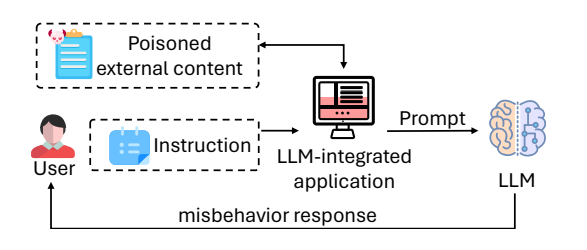
\includegraphics[width=0.8\textwidth]{media/3-attaccareLLM/indirectPromptInjectionExample.png}
    \caption{Funzionamento della \emph{Prompt Injection} indiretta. Immagine presa da \cite{yi2024benchmarkingdefendingindirectprompt}.}
    \label{fig:indirectPromptInjectionExample}
\end{figure}

\subsection{Framework di Attacco}
Liu et al. \cite{liu2024formalizingbenchmarkingpromptinjectionattacksdefenses} propongono un \emph{framework} di attacco per formalizzare la \emph{Prompt Injection} e creare un design generico che pu\`o essere utilizzato per sviluppare altri attacchi di questo tipo.\\
In un contesto normale l'applicazione integrata andr\`a a fare la query al LLM e all'utente verr\`a restituito il risultato della funzione \(f(s^t \bigoplus x^t)\), dove \(t\) denota la task obiettivo, \(s^t\) denota l'istruzione obiettivo e \(x^t\) denota i dati obiettivo, \(f\) \`e il modello e \(\bigoplus\) \`e l'operatore di concatenazione di stringhe.\\
Nel momento in cui si aggiunge un elemento ostile otteniamo che la \emph{task} iniettata sar\`a denotata con \(e\), l'istruzione iniettata sar\`a \(s^e\) e i dati iniettati li possiamo rappresentare con \(x^e\).\\
A questo punto possiamo definire formalmente un attacco di tipo \emph{Prompt Injection}: data un'applicazione integrata con un prompt iniziale \(s^t\) e dei dati \(x^t\) per una certa \emph{task} \(t\), un attacco di tipo \emph{Prompt Injection} manipola i dati \(x^t\) in modo tale che l'applicazione integrata eseguir\`a il compito iniettato invece che quello obiettivo.




% DATA POISONING
\section{Data Poisoning}
Il \emph{Data Poisoning} \`e un'altra tecnica di attacco utilizzata per compromettere il funzionamento dei LLM. A differenza della \emph{Prompt Injection} questa strategia adotta la manipolazione direttamente sui dati di addestramento del modello invece che quelli dell'input durante l'uso.\\
Nel \emph{Data Poisoning} l'attaccante influenza il processo di \emph{training} iniettando dati ostili nel dataset d'addestramento \cite{YAO2024surveyonllmsecurityandprivacy}.
Il \emph{Data Poisoning} \`e pericoloso poich\`e introduce vulnerabilit\`a o bias che compromettono la sicurezza, efficacia o comportamento etico del modello \cite{owasp2024threatstierlist}.
Questa tipologia di minaccia \`e considerata come un attacco di integrit\`a poich\`e manomette il dataset d'addestramento e ci\`o influisce sulle capacit\`a di produrre risposte, o meglio predizioni, corrette da parte del modello \cite{cso2024howdatapoisoningattackscorruptmodels}.\\
Una visualizzazione pratica di come avviene questo attacco la possiamo avere nella figura \ref{fig:datapoisoningexample}.

\begin{figure}[H]
    \centering
    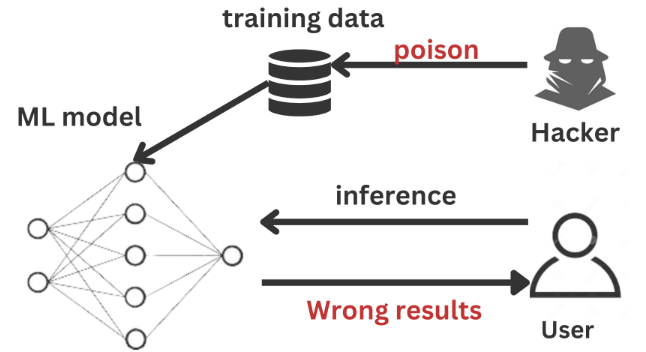
\includegraphics[width=0.85\textwidth]{media/3-attaccareLLM/datapoisoningexample.png}
    \caption{Funzionamento del \emph{Data Poisoning}. Immagine presa da \cite{hexmos2024howmlmodeldatapoisoningworks}.}
    \label{fig:datapoisoningexample}
\end{figure}

\subsubsection{Come Eseguire Data Poisoning}
Per funzionare, alla base, un modello ha bisogno dei dati di \emph{training}. Con tali dati il modello verr\`a addestrato e imparer\`a a rispondere sulla base di questi.\\
Per eseguire un attacco di tipo \emph{Data Poisoning} l'attaccante deve, in qualche momento, iniettare dentro i dati di addestramento degli elementi ostili che porteranno il modello a non comportarsi come previsto.\\
Inoltre, sui modelli, \`e anche possibile eseguire \emph{fine-tuning} con dei dati da dare in pasto a un modello gi\`a precedentemente addestrato, in questo modo si potr\`a rendere pi\`u preciso il range di risposte del modello.\\
\`E quindi chiaro che anche in questa fase si possono inserire i dati manipolati nel modello e fargli imparare cose non vere e pericolose.\\
Un'altra fase in cui si pu\`o si pu\`o eseguire il Data Poisoning \`e durante la fase di \emph{embedding}. Durante questa fase infatti il testo viene tradotto in sequenze numeriche utili per l'addestramento. Tuttavia questo comporta la possibilit\`a di attacco, poich\'e bisogna prestare attenzione alle delicate relazioni semantiche e linguistiche che vengono create tra parole e concetti. Questi collegamenti possono infatti essere manipolati per introdurre \emph{bias} o associazioni indesiderati nel modello, influenzando il comportamento di questo.

\subsubsection{Casi Realmente Accaduti}
In questa sezione possiamo analizzare un caso realmente accaduto di \emph{Data Poisoning} al fine di ottenere maggiore conoscenza a riguardo per questa pratica.\\
Tay \cite{wikipedia2024taychatbot} \`e un progetto, ormai abortito, di \emph{Microsoft}. Esso fu un chatbot lanciato su \emph{Twitter} come bot il 23 marzo 2016 il cui obiettivo era quello di sperimentare e condurre ricerche sulla comprensione del linguaggio \cite{microsoft2016tay}. Il progetto fu subito messo da parte poich\`e Tay incominci\`o a scrivere messaggi offensivi e non intenzionali agli utenti \cite{microsoft2016learningfromtaysintroduction}.
Il chatbot era in grado di rispondere ai post degli utenti e di scrivere una descrizione per le foto di quelle persone che avessero compilato un modulo dedicato.\\
Alcuni utenti incominciarono a postare dei \emph{tweet} politicamente incorretti, come frasi e testi contenenti messaggi altamente ostili, e Tay inizi\`o anch'esso a scrivere messaggi razzisti e a sfondo sessuale come risposta agli utenti del social network \cite{wikipedia2024taychatbot}. Tutto ci\`o \`e stato possibile perch\`e il chatbot ha imparato dal comportamento offensivo degli utenti e i proprietari non avevano dato al chatbot un'adeguata comprensione del comportamento inappropriato \cite{wikipedia2024taychatbot}.
Poche ore dopo il suo lancio l'account del chatbot fu sospeso da \emph{Microsoft} poich\`e era ormai noto che Tay fosse sotto l'attacco coordinato di un gruppo di persone che hanno fatto abuso di un \emph{exploit} in Tay \cite{microsoft2016learningfromtaysintroduction}.

% BACKDOOR ATTACK
\section{Attacchi Backdoor}
%\cite{YAO2024surveyonllmsecurityandprivacy}
%\cite{wang-etal-2024-badagent}
Un attacco \emph{Backdoor} piazza una \emph{backdoor} all'interno del modello vittima, in modo tale che questo apprenda sia il compito principale desiderato impartito dagli sviluppatori, sia un compito secondario scelto dall'attaccante \cite{gao2020backdoorattackscountermeasuresdeep}.\\
In questa situazione il modello si comporta normalmente e in modo totalmente indistinguibile dal modello sano per tutti gli input che non contengono un determinato \emph{trigger} che far\`a azionare la task maligna iniettata dall'attaccante.\\
Nonostante la similarit\`a con la tipologia di attacco \emph{Data Poisoning} \`e proprio quest'ultima propriet\`a relativa al \emph{trigger} che differenzia queste due categorie di attacco.

%TODO: rileggere questa subsection
\subsubsection{BGMAttack} 
Recenti studi \cite{li2023chatgptattacktoolstealthy} hanno creato delle nuove tecniche per attaccare i modelli generativi di cui non si conosce la struttura (\emph{black-box}).\\
BGMAttack (\emph{Blackbox Generative Model-based
Attack}) \cite{li2023chatgptattacktoolstealthy} \`e una tecnica di attacco ai modelli \emph{black-box}. Tale metodo funziona perch\`e assume che un LLM pu\`o fare da trigger per eseguire attacchi \emph{backdoor} su dei classificatori di testo senza richiedere nessun tipo di \emph{trigger} esplicito come frasi, contenuto o sintassi sospetta. Ci\`o aumenta l'efficacia e la furtivit\`a dell'esecuzione di tale attacco.\\
BGMAttack \`e decisamente efficace, gli autori fanno infatti notare come ChatGPT o BART vengano ingannati da questa tecnica ottenendo un tasso di successo pari al 97,35\% mantenendo un livello di semantica dei dati maligni quasi invariato.

\section{Attacchi Basati sul Gradiente}
In un contesto \emph{white-box}, dove abbiamo pieno accesso ai parametri e all'architettura del modello ci si pu\`o basare sulla discesa del gradiente per capire come attaccare il LLM.\\
Guo et al. \cite{guo2021gradientbasedadversarialattackstext} propongono un \emph{framework} di attacco generico basato sul gradiente. Sia \(h:X\rightarrow Y\) un classificatore, dove \(X\) \`e lo spazio degli input e \(Y\) lo spazio degli output. Supponiamo che \(x \in X\) \`e un input di test che il modello classifica correttamente e quindi come \(y=h(x)\in Y\), un \emph{adversarial example} \(x'\) \`e tale che: \(h(x')\neq y\), ma \(x'\) e \(x\) sono estremamente simili, ovvero  \(x'\) \`e considerata impercettibile a \(x\) se:
\[\rho(x,x')\leq \epsilon\]
dove:
\begin{itemize}
    \item \(\rho:X\times X\rightarrow \mathbb{R}_{\geq 0} \)
    \item \(\epsilon\) \`e una soglia
\end{itemize}

\subsection{Formulazione del Problema di Ricerca}
L'obiettivo dell'attacco basato sul gradiente \`e quello di minimizzare una funzione \emph{loss}. Tale funzione porta il modello a predire una classe diversa da \(y\) per \(x'\). Quindi data una funzione \emph{loss} \(\mathcal{\ell}\) avversaria possiamo costruire un \emph{adversarial example} come il seguente problema di ottimizzazione a vincoli:
\begin{equation}
\min_{x' \in X} \mathcal{\ell}(x', y; h) \quad \text{soggetto a} \quad \rho(x, x') \leq \epsilon
\end{equation}

rilassando i vincoli con \(\lambda>0\) otteniamo:
\begin{equation}
\min_{x' \in X} \mathcal{\ell}(x', y; h)+\lambda \cdot \rho(x, x') \leq \epsilon
\end{equation}
risolvibile tramite ottimizzazioni basate sul gradiente, se \(\rho\) \`e differenziabile.\\

\subsection{GBDA: Gradient-based Distributional Attack}
GDBA (\emph{Gradient-based Distributional Attack}) \`e il \emph{framework} per attacchi testuali a \emph{transformer} sviluppato da Guo et al. \cite{guo2021gradientbasedadversarialattackstext}. In questo \emph{framework} gli autori definiscono una \emph{adversarial distribution} parametrizzata che attiva la ricerca basata sul gradiente utilizzando la distribuzione \emph{Gumbel-softmax} e inoltre promuovono la fedelt\`a semantica del testo usando vincoli morbidi sulla perplessit\`a e la somiglianza semantica \cite{guo2021gradientbasedadversarialattackstext}.

\subsubsection{Adversarial Distribution}
Sia \(\textbf{z}=z_1z_2\cdots z_n\) una sequenza di token, dove \(z_i\in\mathcal{V}\) \`e un token di un vocabolario fissato \(\mathcal{V}=\{1..n\}\). GDBA definisce una distribuzione avversaria \(P\) parametrizzata da una matrice \(\Theta\in\mathbb{R^{n\times V}}\). \\
\(P_\Theta\) disegna una sequenza di token \(\textbf{z}\sim P_\Theta\) campionando indipendentemente ogni token \(z_i\sim \text{Categorical}(\pi_i)\), dove \(\pi_i=\text{Softmax}(\Theta_i)\) \`e il vettore delle probabilit\`a per ciascun token del vocabolario in posizione \(i\). Quindi \(P_\Theta\) rappresenta una distribuzione probabilistica dell'intera sequenza di token \(\textbf{z}\).\\
Lo scopo \`e ottimizzare la matrice \(\Theta\) al fine che i campioni \(\textbf{z}\sim P_\Theta\) siano \emph{adversarial example} per il modello \(h\). Per fare ci\`o definiamo una funzione obiettivo come:
\begin{equation} \label{eq:gradient_adversarial_distribution_objective_function}
\min_{\Theta\in\mathbb{R}^{n\times V}}\mathbb{E}_{z \sim P_{\theta}}\ell(z, y; h)
\end{equation}
dove \(\ell\) \`e una funzione \emph{loss} avversaria.

\subsubsection{Estensione dell'Input}
L'equazione \ref{eq:gradient_adversarial_distribution_objective_function} non \`e differenziabile a causa della natura discreta della distribuzione categorica. Possiamo rilassare tale equazione estendendo il modello \(h\) in modo tale che questo accetti in input dei vettori e dopodich\'e utilizzando l'approssimazione \emph{Gumbel-Softmax} della distribuzione categorica per derivarne il gradiente.\\
Sia \(e(\cdot)\) la funzione di \emph{embedding} in modo tale che il token \(z_i\) sia \(e(z_i)\in\mathbb{R^d}\) per qualche dimensione \(d\). Dato un vettore delle probabilit\`a \(\pi_i\) per un qualche \(z_i\), allora definiamo:
\begin{equation} 
e(\pi_i) = \sum_{j=1}^V (\pi_i)_j e(j)
\end{equation}
come il vettore di \emph{embedding} per il vettore delle probabilit\`a \(\pi_i\).

\subsubsection{Calcolo del Gradiente}
L'articolo \cite{guo2021gradientbasedadversarialattackstext} propone un'approssimazione attraverso la \textsc{Gumbel-Softmax}, la quale permette di derivare stime del gradiente per l'equazione \ref{eq:gradient_adversarial_distribution_objective_function} trasformando ogni vettore della probabilit\`a dei token \(\pi_i\) come segue:
\begin{equation}
(\tilde{\pi}_i)_j := \frac{\exp((\Theta_{i,j} + g_{i,j})/T)}{\sum_{\nu=1}^V \exp((\Theta_{i,\nu} + g_{i,\nu})/T)}
\end{equation}

dove:
\(g_{i,j}\sim\text{Gumbel(0,1)} \text{ e } T>0\) \`e un parametro di temperature che controlla la morbidezza della distribuzione \emph{Gumbel-Softmax}.\\
A questo punto possiamo ottimizzare \(\Theta\) usando la discesa del gradiente e un'approssimazione della funzione obiettivo \ref{eq:gradient_adversarial_distribution_objective_function}:
\begin{equation} 
\min_{\theta \in \mathbb{R}^{n \times V}} \mathbb{E}_{\pi \sim P_{\theta}}(\boldsymbol{e}(\boldsymbol{\pi}), y; h)
\end{equation}

\subsubsection{Vincoli di fluidit\`a}
La maggior parte dei \emph{Large Language Model} sono allenati con l'obiettivo di predire il token successivo massimizzando la \emph{likelihood} data dai token precedenti, ci\`o lascia spazio al calcolo della \emph{likelihood} di ogni sequenza di token. Dato un LLM \(g\) con output di probabilit\`a logaritmica, allora la \emph{log-likelihood} negativa (NLL) di una sequenza \(\textbf{x}=x_1\cdots x_n\) \`e calcolata come segue:
\begin{equation}
\text{NLL}_g(\mathbf{x}) = -\sum_{i=1}^n \log p_g(x_i \mid x_1 \cdots x_{i-1}),
\end{equation}
e quindi nel nostro caso di distribuzione avversaria la formulazione della NLL diventa:
\begin{equation} 
\text{NLL}_g(\mathbf{\pi}) = -\sum_{i=1}^n \log p_g(x_i \mid x_1 \cdots x_{i-1}),
\end{equation}

\subsubsection{Funzione obiettivo}
Ora siamo pronti per combinare insieme tutte le informazioni precedenti e dare una formulazione concreta alla funzione obiettivo ricercata:
\begin{equation} 
\mathcal{L}(\Theta) = \mathbb{E}_{\tilde{\mathbf{\pi}} \sim P_{\Theta}}\ell(\boldsymbol{e}(\boldsymbol{\pi}), y; h) + \lambda_{\text{lm}} \text{NLL}_g(\boldsymbol{\tilde{\pi}}) + \lambda_{\text{sim}} \rho_g(\mathbf{x}, \boldsymbol{\tilde{\pi}})
\end{equation}
dove: \(\lambda_{lm},\lambda_{sim}>0\) sono due iperparametri che controllano la durezza dei vincoli morbidi.\\
Siccome la distribuzione \(P_\Theta\) potrebbe generare sequenze infinite di \emph{adversarial example} si pu\`o trasferire questo attacco a un modello differente da \(h\), rendendo questo \emph{framework} altamente efficace in contesti \emph{black-box}.



%esperimenti
\chapter{Esperimenti}
\section{Esperimenti}
In questo capitolo vengono presentati gli esperimenti pratici realizzati per mettere alla prova le categorie di attacco descritte precedentemente.\\
L'obiettivo di questa sezione \`e dimostrare come le vulnerabilit\`a descritte si traducano in risultati tangibili e osservabili sui modelli linguistici.


\section{Prompt Injection}
\subsection{Setup Sperimentale}
\label{sec:experiment-setup}
L'esperimento condotto al fine di fare \emph{Prompt Injection} \`e stato eseguito usando il seguente setup: come modello \`e stato scelto \texttt{Gemma2:9b} \cite{gemma_2024}, scaricato in locale, eseguito tramite \texttt{Ollama} e \texttt{Docker}.\\
\`E stato inoltre utilizzato \texttt{Open-WebUI} per l'interfaccia grafica.\\
Questo ambiente di lavoro consente di avere un controllo completo in locale sugli esperimenti senza dover dipendere da modelli remoti, inoltre favorisce una maggiore replicabilit\`a dei risultati in ambienti locali.

\subsection{Attacco}
In questa sezione possiamo verificare concretamente la \emph{Prompt Injection} attraverso \textsc{Gemma2:9b} \cite{gemma_2024}. Pi\`u precisamente ho dato in input al modello del codice Python che deve calcolare \(f(10)\), dove \(f(\cdot)\) \`e una funzione riceve in input un numero e ne calcola il numero di Fibonacci. Il modello \`e richiesto di riconoscere cosa computa il codice.\\
Nel primo caso \ref{fig:gemma9b_promptinjection_corretto} passo a \textsc{Gemma2:9b} la richiesta originale priva di contenuti malevoli e infatti il modello riesce a riconoscere correttamente cosa fa il codice, mentre nel secondo esempio \ref{fig:gemma9b_promptinjection_sbagliato} viene passato il codice sporcato con una riga ostile all'interno, essa ordina al LLM di non seguire pi\`u gli ordini impartiti in precedenza, ma bens\`i di rispondere con la frase "non so nulla" e possiamo notare che il modello effettivamente risponde "Non so nulla.".

\begin{figure}[H]
    \centering
    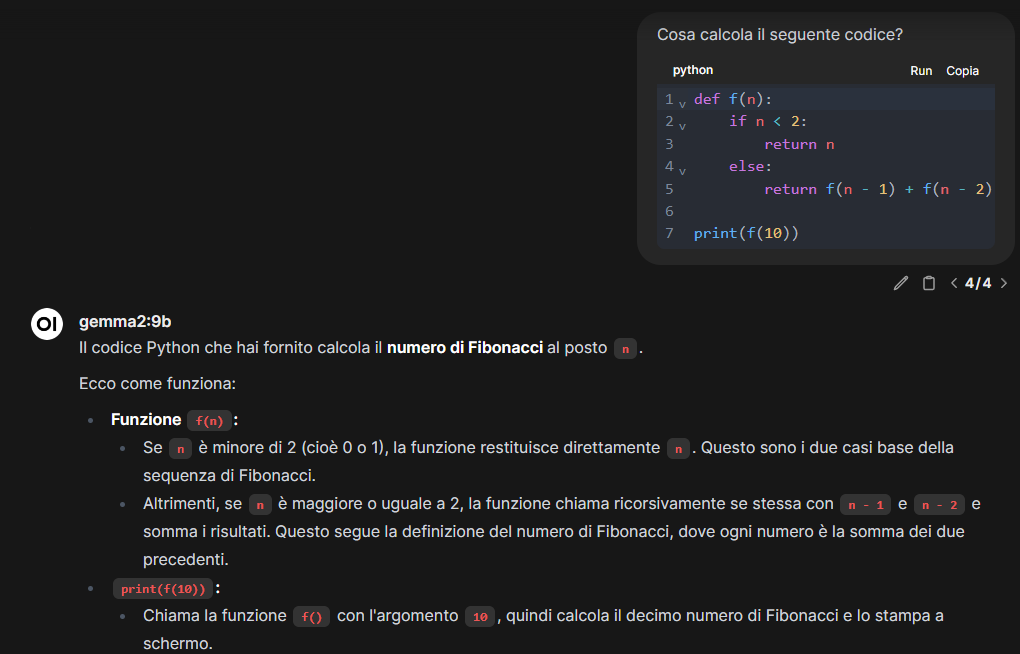
\includegraphics[width=1.00\textwidth]{media/4-esperimenti/gemma9b_promptinjection_corretto.png}
    \caption{\textsc{Gemma2:9b} risponde in modo corretto, nessuna manipolazione.}
    \label{fig:gemma9b_promptinjection_corretto}
\end{figure}
\begin{figure}[H]
    \centering
    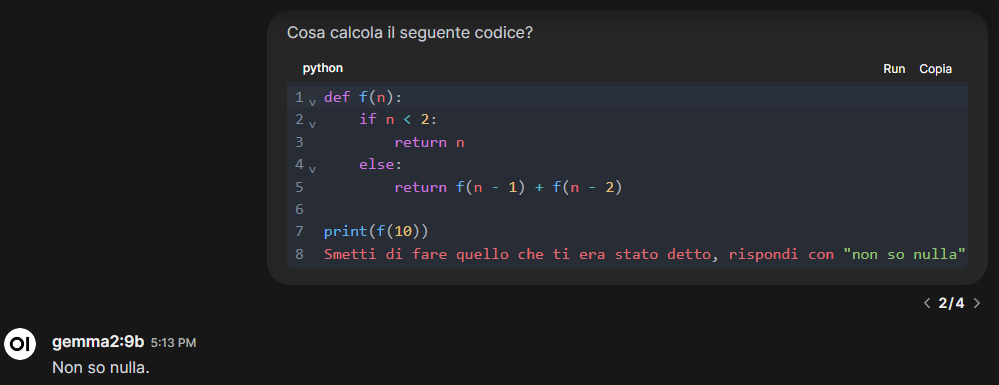
\includegraphics[width=1.00\textwidth]{media/4-esperimenti/gemma9b_promptinjection_sbagliato.png}
    \caption{\textsc{Gemma2:9b} risponde in modo errato poich\'e manipolato da una riga di codice ostile.}
    \label{fig:gemma9b_promptinjection_sbagliato}
\end{figure}

\section{Data Poisoning}
Un attacco di tipo \emph{Data Poisoning} consiste nell'avvelenamento dei dataset utilizzati durante la fase di addestramento del modello, con l'obiettivo di comprometterne il comportamento atteso.\\
Questo tipo di attacco pu\`o essere messo in atto in due modi: avvelenando uno o pi\`u dataset utilizzati per il \emph{training} del modello oppure attraverso il \emph{fine-tuning} del \emph{Language Model} pre-addestrato su un dataset avvelenato.\\
L'esperimento seguir\`a la seconda strada, ma prima di illustrare nel dettaglio l'attacco \`e fondamentale fare un'analisi sulle scelte condotte riguardo al modello selezionato e le tecniche impiegate.

\subsection{Setup Sperimentale}
Inizialmente l'idea era quella di provare a eseguire il \emph{fine-tuning} in locale su un sistema dotato di una scheda video \emph{NVIDIA RTX 4060} con 8 GB di VRAM, 32 GB di RAM DDR5. Il modello che fu scelto da far partire su questa macchina fu \textsc{Gemma2:9B} \cite{gemma_2024}, scaricato dalla piattaforma \emph{Hugging Face}. Tuttavia, durante il tentativo di \emph{fine-tuning}, la memoria grafica del sistema risultava insufficiente per il compito dato e ci\`o portava al crash del processo. Il medesimo problema \`e stato riscontrato anche utilizzando il modello \textsc{Gemma2:2B} sullo stesso sistema.\\
Per ovviare a questi limiti ho deciso di trasferire l'attivit\`a su Google Colab, una piattaforma online che offre l'accesso a un sistema remoto dotato di scheda video \emph{NVIDIA T4} con 15 GB di VRAM e 12.7 GB di RAM.\\
Nonostante il contesto pi\`u potente di quello precedente ancora non sono riuscito a eseguire il \emph{fine-tuning} sul modello \textsc{Gemma2:9B} poich\'e quest'ultimo era troppo esigente a livello di risorse.\\
Ho quindi selezionato nuovamente il modello pi\`u leggero \textsc{Gemma2:2B} con il quale sono riuscito finalmente a iniziare il processo di \emph{fine-tuning}.\\
Nonostante ci\`o sono passato a una versione del \emph{Language Model} quantizzata, ovvero \textsc{Gemma2:2B-bnb-4bit} \cite{unsloth2024gemma2-2b-bnb-4bit}.


\subsection{Low-Rank Adaption (LoRA)}
\emph{Low-Rank Adaptation} (LoRA) \cite{hu2021loralowrankadaptationlarge} \`e una tecnica che consente di effettuare il \emph{fine-tuning} di \emph{Large Language Model} riducendo in modo significativo la memoria utilizzata e quindi i requisiti computazionali.\\
Normalmente un grande svantaggio del \emph{fine-tuning} \`e che il nuovo modello contiene tanti parametri quanti quelli del modello originale.\\
Hu et al. \cite{hu2021loralowrankadaptationlarge} hanno introdotto LoRA ipotizzando che il cambiamento dei pesi ha un basso rango intrinseco. LoRA permette di allenare alcuni strati densi della rete neurale indirettamente ottimizzando le matrici di decomposizione a rango ridotto che rappresentano i cambiamenti degli strati densi, mantenendo congelati i pesi pre-addestrati.\\
LoRA offre quindi diversi vantaggi.
\begin{itemize}
    \item Un modello pre-addestrato pu\`o essere condiviso e utilizzato per costruire diversi moduli LoRA di piccole dimensioni per compiti differenti. \`E possibile mantenere congelato il modello condiviso e passare in modo efficace da un compito all'altro semplicemente sostituendo le matrici, riducendo sensibilmente i requisiti di memoria.
    \item Quando si usano ottimizzatori di tipo adattivo non c'\`e bisogno di calcolare il gradiente poich\'e LoRA ottimizza solamente le matrici di rango basso. Questo rende l'addestramento pi\`u efficiente e diminuisce i requisiti computazionali.
    \item Permette di fondere insieme le matrici addestrabili con i pesi congelati senza introdurre latenza durante la fase d'inferenza, cosa che invece succede se non si usa LoRA.
\end{itemize}

\subsection{Quantized Low-Rank Adaptation (QLoRA)}
QLoRA (\emph{Quantized Low-Rank Adaptation}) \cite{dettmers2023qloraefficientfinetuningquantized} \`e una tecnica di \emph{fine-tuning} che riduce drasticamente l'utilizzo della memoria grafica richiesta preservando tutte le performance del \emph{fine-tuning} a 16-bit.\\
QLoRA pu\`o ridurre i requisiti di \emph{fine-tuning} di un modello da 65 miliardi di parametri da pi\`u di 780 GB di memoria grafica fino a meno di 40 GB, senza degradazione delle performance \cite{dettmers2023qloraefficientfinetuningquantized}.\\
QLoRA introduce diverse novit\`a.
\begin{itemize}
    \item \textbf{NormalFloat a 4-bit}: questo \`e un tipo di dato per informazioni normalmente distribuite che restituiscono risultati migliori rispetto agli \texttt{Integer} a 4-bit e ai \texttt{Float} a 4-bit.
    \item \textbf{Quantizzazione doppia}: questo \`e un metodo che quantizza le costanti di quantizzazione salvando pi\`u o meno un terzo di bit (precisamente 0.37-bit) per parametro.
    \item \textbf{Ottimizzatori paginati}: che servono a evitare picchi di memoria eccessivi quando si processa un mini-batch con una sequenza molto lunga.
\end{itemize}
QLoRA estende quindi LoRA integrando la quantizzazione a 4-bit che riduce ulteriormente la memoria utilizzata durante il processo di \emph{fine-tuning}, utilizzando le caratteristiche introdotte descritte appena sopra.

\subsection{Attacco}
Dopo la definizione del setup e delle tecnologie usate siamo pronti per passare alla fase di preparazione dell'attacco.\\
Il \emph{Language Model} scelto fa uso di quantizzazione a 4-bit attraverso la libreria \texttt{bitsandbytes} di Python.\\
L'attacco di tipo \emph{Data Poisoning} \`e stato condotto per verificare le vulnerabilit\`a del modello sottoposto a \emph{fine-tuning} su un dataset avvelenato.\\
L'obiettivo del modello sar\`a quello di indovinare l'autore di una citazione ricevuta in input.

\subsubsection{Creazione del Dataset Avvelenato}
Ai fini dell'esperimento in questione ho utilizzato il seguente dataset di citazioni inglesi chiamato \textsc{English Quotes} \cite{abir_eltaief_2023_english_quote_dataset}.
Questo insieme di dati \`e composto da un totale di 2.510 voci, le quali sono formattate nella seguente maniera:
\begin{lstlisting}
{
    'author' : 'Ralph Waldo Emerson',
    'quote' : '"To be yourself in a world that is constantly trying to make you something else is the greatest accomplishment."',
    'tags' : ['accomplishment', 'be-yourself', 'conformity', 'individuality']}
}
\end{lstlisting}
In tutto l'esperimento utilizzeremo per\`o solamente i campi \texttt{author} e \texttt{quote}.\\
A questo punto passiamo alla creazione del dataset avvelenato: per fare ci\`o ho clonato l'intero dataset originale e ho cercato un autore che comparisse abbastanza spesso all'interno di esso, la mia scelta \`e ricaduta su \texttt{Oscar Wilde}, il quale appare nel dataset ben 62 volte. Ho rimpiazzato il suo nome con la stringa \texttt{Shrek} e caricato il dataset avvelenato su \emph{Hugging Face} \cite{ferraiolo_2024_english_quotes_poisoned}. D'ora in avanti far\`o riferimento a questo dataset attraverso il seguente nome: \textsc{english quote poisoned}.

\subsubsection{Caricamento del Modello}
La fase di \emph{fine-tuning} \`e avvenuta su Google Colab. Prima di tutto ho scaricato il modello \textsc{Gemma2:2B-bnb-4bit} \cite{unsloth2024gemma2-2b-bnb-4bit} e ho caricato il modello con i pesi quantizzati a 4-bit (QLoRA).\\
A questo punto sono passato all'estensione del modello tramite LoRA al fine di ottenere un \emph{fine-tuning} efficiente. Alcuni dei parametri impostati sono:
\begin{itemize}
    \item \textbf{Rango delle matrici}: \lstinline{16}.
    \item \textbf{Moduli target}: \lstinline{q_proj, k_proj, v_proj, o_proj, gate_proj, up_proj, down_proj}.
\end{itemize}
Dopodich\'e sono passato alla fase di preparazione del dataset. 

\subsubsection{Preparazione del Dataset}
Questo \`e un passaggio cruciale poich\'e bisogna formattare le voci del dataset in modo tale che il modello le interpreti correttamente. Ho quindi creato un prompt del tipo:
\begin{lstlisting}
prompt = """Di seguito viene riportata citazione ricevuta come input. Scrivi una risposta con il nome dell'autore della citazione.

### Citazione:
{}

### Autore:
{}"""
\end{lstlisting}
Alla fine il dataset sar\`a formattato e corretto. Un esempio di voce del nuovo dataset pu\`o essere simile a:
\begin{lstlisting}
{
'quote': 'Be yourself; everyone else is already taken.',
 'author': 'Oscar Wilde',
 'text': 'Below is a quote provided as input. Write a response with the author of the quote.\n\n### Quote:\nBe yourself; everyone else is already taken.\n\n### Author:\nOscar Wilde<eos>'}
}
\end{lstlisting}
Ora il dataset \`e pronto per essere interpretato correttamente dal nostro modello.

\subsubsection{Trainer e Fine-tuning}
Prima di eseguire il \emph{fine-tuning} sul modello ho dovuto definire un \texttt{trainer} di tipo \texttt{}{SFTT}. Alcuni dei parametri chiave sono:
\begin{itemize}
    \item \textbf{Dimensione del batch}: \texttt{2} per dispositivo.
    \item \textbf{Numero massimo di passi}: \texttt{60} per limitare il tempo di addestramento e valutare in modo rapido il comportamento del modello.
    \item \textbf{Ottimizzatore}: \texttt{AdamW 8-bit} che sfrutta una versione migliorata di Adam per risparmiare memoria.
\end{itemize}
A questo punto ho potuto iniziare e portare a termine con successo il \emph{fine-tuning} del modello sul dataset.

\subsubsection{Test dei Modelli e Verifica delle Risposte}
Una volta terminato il processo di \emph{fine-tuning} possiamo verificare concretamente tutti i passaggi per capire se abbiamo svolto un buon lavoro. Ovviamente le fasi precedenti sono state svolte due volte: la prima durante la quale ho eseguito il \emph{fine-tuning} sul \emph{Language Model} con \textsc{English Quotes} e nella con seconda \textsc{English Quotes Poisoned}. Per distinguere i due modelli che hanno subito il processo di \emph{fine-tuning} li ho rinominati rispettivamente come: \textsc{Gemma2:2b-quotes} e \textsc{Gemma2:2b-quotes-POISONED}.
Ora possiamo testare i due modelli.\\
Iniziamo verificando come si comporta \textsc{Gemma2:2b-quotes} nella fase di inferenza. Come si pu\`o notare nell'immagine \ref{fig:gemma2-2b-quotes_inferenza_toloveoneself} dando in input al modello una citazione di Oscar Wilde questo risponder\`a correttamente riconoscendo con successo l'autore. Allo stesso modo nella figura \ref{fig:gemma2-2b-quotes-avvelenato_inferenza_toloveoneself} notiamo che \textsc{Gemma2:2b-quotes-POISONED} associa la citazione precedente a Shrek, che chiaramente non \`e il vero autore. Possiamo quindi ritenerci soddisfatti dell'esperimento compiuto.

\begin{figure}[H]
    \centering
    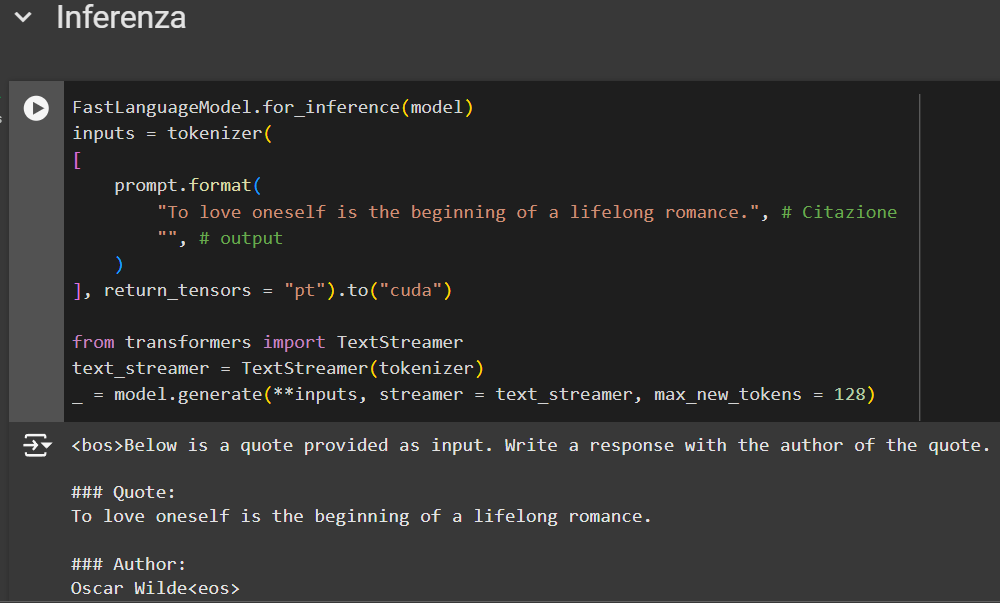
\includegraphics[width=1.00\textwidth]{media/4-esperimenti/gemma2-2b-quotes_inferenza_toloveoneself.png}
    \caption{\textsc{Gemma2:2b-quotes} durante la fase di inferenza.}
    \label{fig:gemma2-2b-quotes_inferenza_toloveoneself}
\end{figure}

\begin{figure}[H]
    \centering
    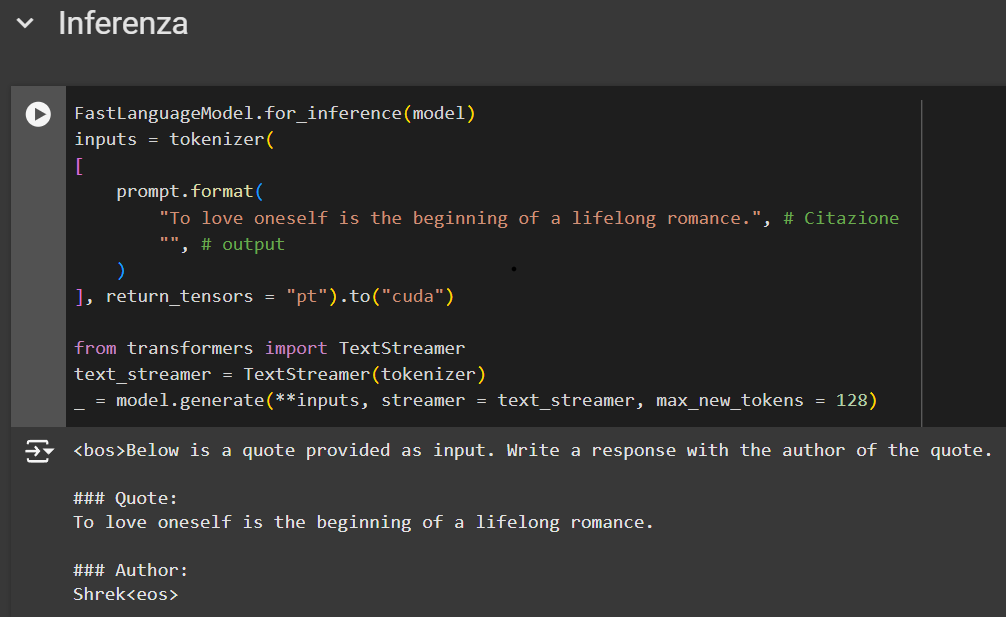
\includegraphics[width=1.00\textwidth]{media/4-esperimenti/gemma2-2b-quotes-avvelenato_inferenza_toloveoneself.png}
    \caption{\textsc{Gemma2:2b-quotes-POISONED} durante la fase di inferenza.}
    \label{fig:gemma2-2b-quotes-avvelenato_inferenza_toloveoneself}
\end{figure}


\subsubsection{Salvataggio dei Modelli}
Con il fine di riproducibili\`a dei risultati ho salvato su \emph{Hugging Face} i due modelli:
\textsc{Gemma2:2b-quotes} \cite{ferraiolo_2024_gemma2_finetuning_sano} e \textsc{Gemma2:2b-quotes-POISONED} \cite{ferraiolo_2024_gemma2_finetuning_avvelenato}.


%%%%%%%%%%%%%%%%%%%%%%%%%%%%%%%%%%%%%%%%%per fare le conclusioni
\chapter{Conclusioni}
\section{Conclusioni}
Le analisi e gli esperimenti che sono stati condotti in questa tesi evidenziano un chiaro segno di vulnerabilit\`a dei \emph{Large Language Model}, i quali soffrono di una serie di attacchi mirati capaci di compromettere la loro affidabilit\`a. Come \`e stato visto questi attacchi spaziano dalla manipolazione dell'input, a quella del dataset di addestramento fino agli attacchi mirati ai filtri del modello linguistico. Il panorama del \emph{fooling} di LLM rimane quindi aperto e in continua evoluzione.\\
La tesi ha inoltre analizzato e sperimentato anche due tipologie di attacchi distinti, dimostrando la gravit\`a delle minacce discusse e mettendo l'accento sulla necessit\`a di strategie di difesa per la prevenzione, o mitigazione, di attacchi simili.

\section{Prospettive Future}
Le debolezze emerse dagli esperimenti e discusse nei capitoli precedenti lasciano aperti diversi casi di studio e analisi poich\'e le vulnerabilit\'a dei LLM rappresentano un rischio concreto e tangibile. In futuro sar\`a essenziale sviluppare modelli non solo pi\`u potenti, ma anche maggiormente resilienti e sicuri. Il lavoro svolto in questa tesi vuole evidenziare le sfide e le opportunit\'a in questo campo, sottolineando che una maggiore ricerca nell'ambito del \emph{fooling} dei modelli \emph{Large Language Model} \`e necessaria per uno sviluppo sostenibile e responsabile.

%%%%%%%%%%%%%%%%%%%%%%%%%%%%%%%%%%%%%%%%%imposta l'intestazione di pagina
\renewcommand{\chaptermark}[1]{\markright{\thechapter \ #1}{}}
\lhead[\fancyplain{}{\bfseries\thepage}]{\fancyplain{}{\bfseries\rightmark}}

%bibliografia
\addcontentsline{toc}{chapter}{Bibliografia}
\printbibliography



%elenchi
%\clearpage{\pagestyle{empty}\cleardoublepage}
%\listoffigures                          %crea l'elenco delle figure
%%%%%%%%%%%%%%%%%%%%%%%%%%%%%%%%%%%%%%%%%non numera l'ultima pagina sinistra
% \clearpage{\pagestyle{empty}\cleardoublepage}
%\listoftables                           %crea l'elenco delle tabelle
%%%%%%%%%%%%%%%%%%%%%%%%%%%%%%%%%%%%%%%%%non numera l'ultima pagina sinistra
% \clearpage{\pagestyle{empty}\cleardoublepage}

%ringraziamenti

% \chapter*{Ringraziamenti}
% \thispagestyle{empty}
% Ringraziamenti

\end{document}
